%==============================================================================
% Makalah Gemastik — Buletin Pagelaran Mahasiswa Nasional Bidang TIK
% Judul: Peningkatan Keandalan dan Efisiensi Token LLM pada Data Time Series
%        melalui Pendekatan Verifikasi Deterministik
% Kompilasi: pdflatex 02_KrocoMasStanis.tex  (jalankan 2x untuk referensi)
% Berkas gambar: arsitektur_sistem.png, plot_rq2.png (folder sama)
% Figur dari data eksperimen asli: python experiments/plot_paper_figs.py
%==============================================================================
\documentclass[10pt,a4paper,twocolumn]{article}

\usepackage[T1]{fontenc}
\usepackage[utf8]{inputenc}
% babel[indonesian] sengaja TIDAK dipakai: banyak instalasi TeX Live tidak
% menyertakan indonesian.ldf sehingga kompilasi gagal total. Babel bahasa
% Indonesia hanya memengaruhi nama otomatis (label caption / referensi) yang
% sudah di-override manual di bawah, jadi tidak dibutuhkan secara fungsional.
\usepackage{mathptmx}            % Times New Roman untuk teks & matematika
\usepackage[scaled=0.92]{helvet} % Helvetica Type1 asli (hindari fallback bitmap)
\usepackage{amsmath,amssymb}
\usepackage{graphicx}
\usepackage{booktabs}
\usepackage{array}
\usepackage{ragged2e}
\usepackage{caption}
\usepackage{fancyhdr}
\usepackage{url}
\usepackage[hidelinks]{hyperref}
\usepackage[a4paper,left=1.8cm,right=1.8cm,top=2.6cm,bottom=2.2cm,%
            columnsep=0.7cm,headsep=0.5cm]{geometry}

%------------------------------------------------------------------------------
% Penomoran bagian: I., A. (IEEE style)
%------------------------------------------------------------------------------
\renewcommand{\thesection}{\Roman{section}}
\renewcommand{\thesubsection}{\Alph{subsection}}

% Gaya heading IEEE tanpa titlesec (paket titlesec tidak ada di sebagian
% instalasi TeX Live). Reproduksi dengan \@startsection base LaTeX:
% Level 1 = kecil, bold, "I." + spasi; Level 2 = kecil, bold-italic, "A.".
\makeatletter
\renewcommand{\@seccntformat}[1]{\csname the#1\endcsname.\hspace{0.5em}}
\renewcommand\section{\@startsection{section}{1}{\z@}%
  {1.4ex \@plus .3ex}{0.8ex}%
  {\normalfont\small\bfseries}}
\renewcommand\subsection{\@startsection{subsection}{2}{\z@}%
  {1.2ex \@plus .2ex}{0.6ex}%
  {\normalfont\small\bfseries\itshape}}
\makeatother

%------------------------------------------------------------------------------
% Gaya caption
%------------------------------------------------------------------------------
\captionsetup{font=small,labelsep=period,justification=centering}
\captionsetup[table]{font=footnotesize,labelfont=bf,skip=3pt}
\captionsetup[figure]{font=small,skip=4pt}

% Nama otomatis bahasa Indonesia (menggantikan peran babel yang dilepas di atas)
\renewcommand{\figurename}{Gambar}
\renewcommand{\tablename}{Tabel}
\renewcommand{\refname}{REFERENSI}

%------------------------------------------------------------------------------
% Header banner + footer
%------------------------------------------------------------------------------
\setlength{\headheight}{26pt}
\pagestyle{fancy}
\fancyhf{}
\renewcommand{\headrulewidth}{0.8pt}
\renewcommand{\footrulewidth}{0pt}
\fancyhead[L]{%
  \footnotesize\bfseries BULETIN PAGELARAN MAHASISWA NASIONAL BIDANG TEKNOLOGI INFORMASI DAN KOMUNIKASI\\%
  \mdseries\scriptsize ISSN: xxxxxx}
\fancyfoot[L]{\footnotesize Ketua Tim: Peningkatan Keandalan dan Efisiensi \ldots}
\fancyfoot[R]{\footnotesize Volume 1 Nomor 1 September 2024}

\setlength{\parindent}{1.2em}
\setlength{\parskip}{0pt}

\begin{document}

%==============================================================================
% JUDUL, PENULIS, INTISARI (lebar penuh)
%==============================================================================
\twocolumn[{%
\begin{@twocolumnfalse}
\thispagestyle{fancy}
\vspace{0.5em}
\begin{center}
  {\LARGE\bfseries Peningkatan Keandalan dan Efisiensi Token LLM pada Data
   Time Series melalui Pendekatan Verifikasi Deterministik\par}
  \vspace{1.2em}
  {\normalsize Ahmad Naufal Farras\textsuperscript{1}, Jeremy Mattathias
   Mboe\textsuperscript{2}, Mochammad Henry Alifian\textsuperscript{3},
   Dhany Arifianto\textsuperscript{4}\par}
  \vspace{0.6em}
  {\footnotesize
   \textsuperscript{1}Fakultas Teknologi Elektro dan Informatika Cerdas,
   Institut Teknologi Sepuluh Nopember, Surabaya, 60111,
   email: 5054241038@student.its.ac.id\\
   \textsuperscript{2}Fakultas Teknologi Elektro dan Informatika Cerdas,
   Institut Teknologi Sepuluh Nopember, Surabaya, 60111,
   email: 5054241021@student.its.ac.id\\
   \textsuperscript{3}Fakultas Teknologi Elektro dan Informatika Cerdas,
   Institut Teknologi Sepuluh Nopember, Surabaya, 60111,
   email: 5054241024@student.its.ac.id\\
   \textsuperscript{4}Fakultas Kedokteran dan Kesehatan,
   Institut Teknologi Sepuluh Nopember, Surabaya, 60111\\[0.3em]
   \textit{Corresponding Author}: Ahmad Naufal Farras\par}
\end{center}
\vspace{0.6em}

{\small\justifying
\noindent\textbf{\textit{INTISARI}} --- \textit{Large language model} (LLM)
unggul mengolah bahasa alami, tetapi keandalannya menurun ketika penalaran
menuntut komputasi numerik atas data \textit{time series}. Karena bekerja dengan
memprediksi \textit{token} berikutnya berdasarkan pola kebahasaan, model
cenderung mengira-ngira alih-alih menghitung, sehingga kesimpulan dapat keliru
meski kalimatnya meyakinkan. Pada domain berisiko tinggi seperti kesehatan
masyarakat dan pangan, penalaran semacam ini dituntut dapat diaudit, yakni setiap
angka pada tiap langkah dapat diperiksa ulang atau \textit{grounded}. Namun dua
kelompok metode yang ada saling bertolak belakang: penalaran terverifikasi
bersifat boros \textit{token}, sedangkan penalaran hemat \textit{token} hanya
menjaga akurasi jawaban tanpa memeriksa kesahihan langkah antaranya. Penelitian
ini bertujuan menutup celah tersebut melalui pendekatan yang memisahkan penalaran
menjadi dua komponen: LLM hasil \textit{fine-tune} kelas Qwen2.5-7B yang
menuliskan penalaran sebagai urutan \textit{operasi} dari pustaka tetap, dan
verifikator deterministik berbasis NumPy yang menghitung ulang serta memeriksa
tiap operasi terhadap deret asli. Skor \textit{grounding} dihitung tanpa penilai
LLM dan dilaporkan bersama akurasi jawaban dan jumlah \textit{token}.
\textit{Dataset} dibangun dari sumber publik Indonesia, yaitu deret nyata Badan
Pusat Statistik untuk data latih dan World Bank Open Data untuk data uji, dengan
label bersih \textit{by construction} karena disaring verifikator di dalam
\textit{loop}. Hasil uji pada tiga model tanpa \textit{fine-tune} memperlihatkan
skor \textit{grounding} yang rendah (2--16\%) meski akurasi jawaban cukup, dan
ketika penalaran dipendekkan untuk menghemat \textit{token}, skor
\textit{grounding} menurun lebih cepat daripada akurasi hingga mendekati nol.
Verifikator tervalidasi dengan skor \textit{grounding} 100\% pada penalaran valid
dan 66,7\% saat halusinasi disuntikkan, lolos 139 pengujian otomatis, dan
disepakati 471 dari 471 langkah oleh jalur perhitungan independen. Kebaruan
penelitian terletak pada temuan tarik-menarik \textit{grounding} lawan
\textit{token} dan pada mekanisme efisiensi yang sadar \textit{grounding}, bukan
sekadar penggabungan dua pendekatan.
\par\vspace{0.7em}
\noindent\textbf{KATA KUNCI:} \textit{Grounded Reasoning}, \textit{Time Series},
Skor \textit{Grounding}, Verifikator Deterministik, Efisiensi \textit{Token},
\textit{Chain-of-Thought}, \textit{Fine-tuning} LLM, QLoRA, Penalaran
Neuro-Simbolik.
\par}
\vspace{0.6em}
\end{@twocolumnfalse}
}]

%==============================================================================
% ISI (dua kolom)
%==============================================================================
\justifying

\section{PENDAHULUAN}
Data \textit{time series} menempati inti banyak keputusan penting --- kasus
penyakit yang dilaporkan tiap minggu, harga pangan yang dipantau tiap hari, dan
beban energi yang tercatat tiap jam --- sehingga kemampuan menafsirkan deret
angka secara benar bernilai tinggi. \textit{Large language model} (LLM)
menjanjikan antarmuka yang luwes untuk penafsiran tersebut, tetapi keandalannya
menurun tajam saat persoalan bergeser dari bahasa ke bilangan. Akar persoalannya
bersifat teoretis: LLM dilatih memprediksi \textit{token} berikutnya berdasarkan
pola kebahasaan, sehingga ketika diberi sederet angka ia cenderung mereproduksi
pola yang lazim menyertai angka serupa alih-alih melakukan komputasi sebenarnya.
Studi mutakhir menegaskan bahwa model masih kesulitan menalar \textit{time
series} bahkan pada pengaturan \textit{zero-shot}~\cite{merrill2024,mtbench2025}.
Sebagai ilustrasi, pada deret kasus demam berdarah selama 16 minggu $12, 15, 11,
14, 13, 18, 22, 19, 25, 31, 29, 38, 45, 52, 61, 78$, model kerap menyimpulkan
kondisi stabil padahal nilai akhir mencapai sekitar enam kali garis dasar, salah
menunjuk minggu terjadinya lonjakan, atau menyebut kenaikan 30\% padahal
mendekati 105\%.

Upaya baku mengatasi kelemahan ini adalah memperpanjang penalaran melalui
\textit{Chain-of-Thought} (CoT)~\cite{cot2022} dan memindahkan komputasi ke
program pada \textit{Program-of-Thought} (PoT)~\cite{pal2023}. Pendekatan tersebut
kerap menaikkan akurasi jawaban, namun menyisakan celah yang lebih mendasar:
akurasi jawaban adalah proksi yang lemah bagi kualitas penalaran. Sebuah model
dapat menghasilkan jawaban benar melalui langkah-langkah antara yang keliru ---
benar karena alasan yang salah --- dan selama langkah tersebut ditulis sebagai
prosa bebas, kekeliruannya tidak dapat diperiksa. Dengan kata lain, memperpanjang
penalaran tidak dengan sendirinya membuatnya \textit{grounded}, yaitu membuat tiap
angka pada tiap langkah dapat dihitung ulang dan diverifikasi terhadap deret asli.

Kebutuhan akan penalaran yang \textit{grounded} justru berbenturan dengan
kebutuhan akan efisiensi, dan di sinilah letak celah yang belum terpecahkan. Di
satu sisi, metode penalaran terverifikasi untuk \textit{time series} seperti
VeriTime~\cite{veritime2026} menjamin kesahihan langkah namun menghasilkan
penalaran panjang yang boros \textit{token}. Di sisi lain, metode hemat
\textit{token} seperti SelfBudgeter~\cite{selfbudgeter2025} mengatur anggaran
penalaran demi efisiensi, tetapi mengoptimalkan akurasi jawaban semata tanpa
pernah memeriksa kesahihan langkah antaranya. Penerjemahan langkah penalaran ke
representasi formal yang dieksekusi \textit{solver} deterministik terbukti efektif
mengeliminasi halusinasi logika~\cite{logiclm2023}, namun belum diarahkan pada
tarik-menarik antara \textit{grounding} dan biaya \textit{token} pada
\textit{time series}. Konsekuensinya adalah tarik-menarik yang selama ini luput:
ketika penalaran dipendekkan untuk menghemat \textit{token}, skor \textit{grounding}
dapat menurun lebih cepat daripada akurasi jawaban, sehingga penalaran kehilangan
keterandalannya tanpa terdeteksi oleh metrik yang hanya memantau jawaban akhir.
Menjaga \textit{grounding} tetap tinggi di bawah anggaran \textit{token} ---
khususnya pada \textit{time series} --- dengan demikian merupakan masalah terbuka.

Taruhan celah ini nyata pada domain berisiko tinggi. Model yang menyimpulkan
tren datar padahal kasus melonjak enam kali lipat dapat menunda respons wabah,
dan kesalahan menaksir besaran kenaikan harga --- misalnya melaporkan 30\%
alih-alih 105\% --- dapat memicu intervensi kebijakan yang keliru sasaran. Pada
konteks demikian, sebuah jawaban tidak cukup benar; jejak penalarannya harus
dapat diaudit angka demi angka oleh pengambil keputusan. Persoalan ini kian
mengemuka di Indonesia, yang kaya sumber data publik tetapi belum memiliki
\textit{dataset} penalaran \textit{time series} terverifikasi berbahan sumber
lokal sebagai landasan pengembangan dan evaluasi.

Untuk menjawab persoalan tersebut, diusulkan pendekatan yang secara arsitektural
memisahkan tanggung jawab: komponen model berupa LLM hasil \textit{fine-tune}
menuliskan penalaran sebagai urutan \textit{operasi} dari pustaka tetap alih-alih
prosa bebas, sedangkan komponen program berupa verifikator deterministik
menghitung ulang tiap \textit{operasi} atas deret asli dan memeriksa kesesuaiannya
dalam toleransi. Dengan pemisahan ini, model tidak pernah memegang kepemilikan
atas angka; angka dihitung dan diperiksa oleh program di luar model, sehingga
penalaran tetap dapat diaudit. Di atas fondasi tersebut dirancang mekanisme
penalaran adaptif yang sadar \textit{grounding}, yang menargetkan rantai
\textit{operasi} ter-\textit{grounded} terpendek yang memadai untuk tiap
persoalan, sehingga efisiensi dan \textit{grounding} dioptimalkan bersama.
Kontribusi penelitian ini ada tiga dan saling menopang: pertama, temuan empiris
mengenai tarik-menarik \textit{grounding} lawan \textit{token}; kedua,
\textit{dataset} penalaran \textit{time series} terverifikasi dari sumber publik
Indonesia; dan ketiga, metrik skor \textit{grounding} deterministik yang dihitung
tanpa penilai LLM. Sesuai uraian tersebut, penelitian ini menjawab empat
pertanyaan penelitian: \textbf{RQ1}, seberapa sering model saat ini menghasilkan
penalaran ber-\textit{grounding} rendah walau jawabannya kadang benar;
\textbf{RQ2}, apakah \textit{grounding} menurun lebih cepat daripada akurasi
ketika penalaran dipendekkan; \textbf{RQ3}, apakah pendekatan yang diusulkan
mempertahankan \textit{grounding} pada anggaran \textit{token} yang jauh lebih
hemat; dan \textbf{RQ4}, berapa sumbangan tiap komponen terhadap kinerja
keseluruhan.

\section{TINJAUAN PUSTAKA}

\subsection{Penalaran atas Time Series}
Model bahasa besar masih sulit menalar \textit{time series} tanpa contoh, dan
penalaran yang panjang tidak selalu menaikkan mutu analisis deret
waktu~\cite{merrill2024}. Tolok ukur multimodal untuk penalaran temporal
memperlihatkan model masih gagal ketika harus menggabungkan angka dan
teks~\cite{mtbench2025}. Sejumlah karya terkini mendorong penalaran yang lebih
rumit atas \textit{time series} melalui pelatihan berbasis
insentif~\cite{timeomni2026}. Kumpulan karya ini menunjukkan bidangnya aktif
tetapi belum tuntas, khususnya pada aspek keterandalan langkah antaranya.

\subsection{Chain-of-Thought dan Program-of-Thought}
Memunculkan langkah penalaran antara terbukti menaikkan hasil pada tugas rumit,
tetapi langkah itu tetap berupa prosa yang bisa salah hitung~\cite{cot2022}.
Pemindahan komputasi ke penafsir program membuat jawaban dihitung alih-alih
ditebak~\cite{pal2023}. Integrasi fungsional antara LLM dan \textit{interpreter}
eksternal, seperti pada ToRA, terbukti secara masif mengoreksi galat komputasi
kompleks melalui eksekusi kode terstruktur~\cite{tora2024}. Penelitian ini memakai
semangat yang sama: LLM tidak pernah memegang angka, ia hanya mengusulkan
\textit{operasi}, dan program di luar model yang menghitung dan mengecek.

\subsection{Penalaran Terverifikasi untuk Time Series}
Arah yang paling dekat dengan penelitian ini menggarap penalaran \textit{time
series} yang dapat diverifikasi melalui sintesis dan penjadwalan data berpikir,
yang dikenal sebagai VeriTime~\cite{veritime2026}. Penelitian ini diletakkan
langsung terhadap arah tersebut, dengan pembeda menggabungkan penalaran
terverifikasi dan hemat \textit{token} serta membangun data sendiri dari konteks
lokal, dan tidak menyandarkan kontribusi pada klaim bahwa arah terverifikasi
selalu mahal.

\subsection{Efisiensi Token dan Penalaran Adaptif}
Panjang penalaran dapat dibuat hemat dan menyesuaikan tingkat kesulitan lewat
pengaturan anggaran \textit{token}, meski sejauh ini terbatas pada soal
matematika~\cite{selfbudgeter2025}. Alokasi anggaran komputasi yang adaptif
berdasarkan kompleksitas masukan terbukti mampu memangkas biaya penggunaan
\textit{token} secara signifikan tanpa mengorbankan akurasi akhir
sistem~\cite{frugalgpt2023}. Gagasan anggaran adaptif itu dipinjam dan dibawa ke
ranah \textit{time series}, yang belum pernah dilakukan.

\subsection{Pelatihan Hemat Sumber Daya}
\textit{Low-Rank Adaptation} (LoRA)~\cite{lora2022} dan kuantisasi NF4 4-bit pada
QLoRA~\cite{qlora2023} memungkinkan penyetelan model kelas 7B pada GPU T4 atau
V100. Karena kekuatan proyek ada pada data dan \textit{grounding}, model kelas 7B
seperti Qwen2.5~\cite{qwen2024} dinilai memadai. Posisi penelitian ini terhadap karya
terkait diringkas pada Tabel~\ref{tab:posisi}.

\begin{table}[t]
\centering
\caption{Posisi Penelitian Ini terhadap Karya Terkait}
\label{tab:posisi}
\footnotesize
\begin{tabular}{@{}lcccc@{}}
\toprule
\textbf{Karya} & \textbf{Terverif.} & \textbf{Hemat} & \textbf{\textit{Time}} & \textbf{Data} \\
 & & \textbf{\textit{token}} & \textbf{\textit{series}} & \textbf{lokal} \\
\midrule
CoT / PoT~\cite{cot2022,pal2023} & sebagian & tidak & tidak & -- \\
SelfBudgeter~\cite{selfbudgeter2025} & tidak & ya & tidak & -- \\
VeriTime~\cite{veritime2026} & ya & tidak & ya & tidak \\
Usulan ini & ya & ya & ya & ya \\
\bottomrule
\end{tabular}
\end{table}

\section{METODOLOGI}

\subsection{Gambaran Sistem}
Alur inti sistem berjalan sebagai berikut. LLM menerima deret angka beserta
pertanyaan, lalu menuliskan penalaran dalam bentuk langkah beroperasi, bukan
prosa bebas. Verifikator deterministik di luar model kemudian menghitung ulang
tiap operasi atas deret asli dan mengecek angka yang diklaim cocok dalam
toleransi. Keduanya benda terpisah yang bekerja bersama, bukan program yang
ditanam ke dalam LLM. Gambaran alur ini ada pada Gambar~\ref{fig:arsitektur}.

\begin{figure}[t]
\centering
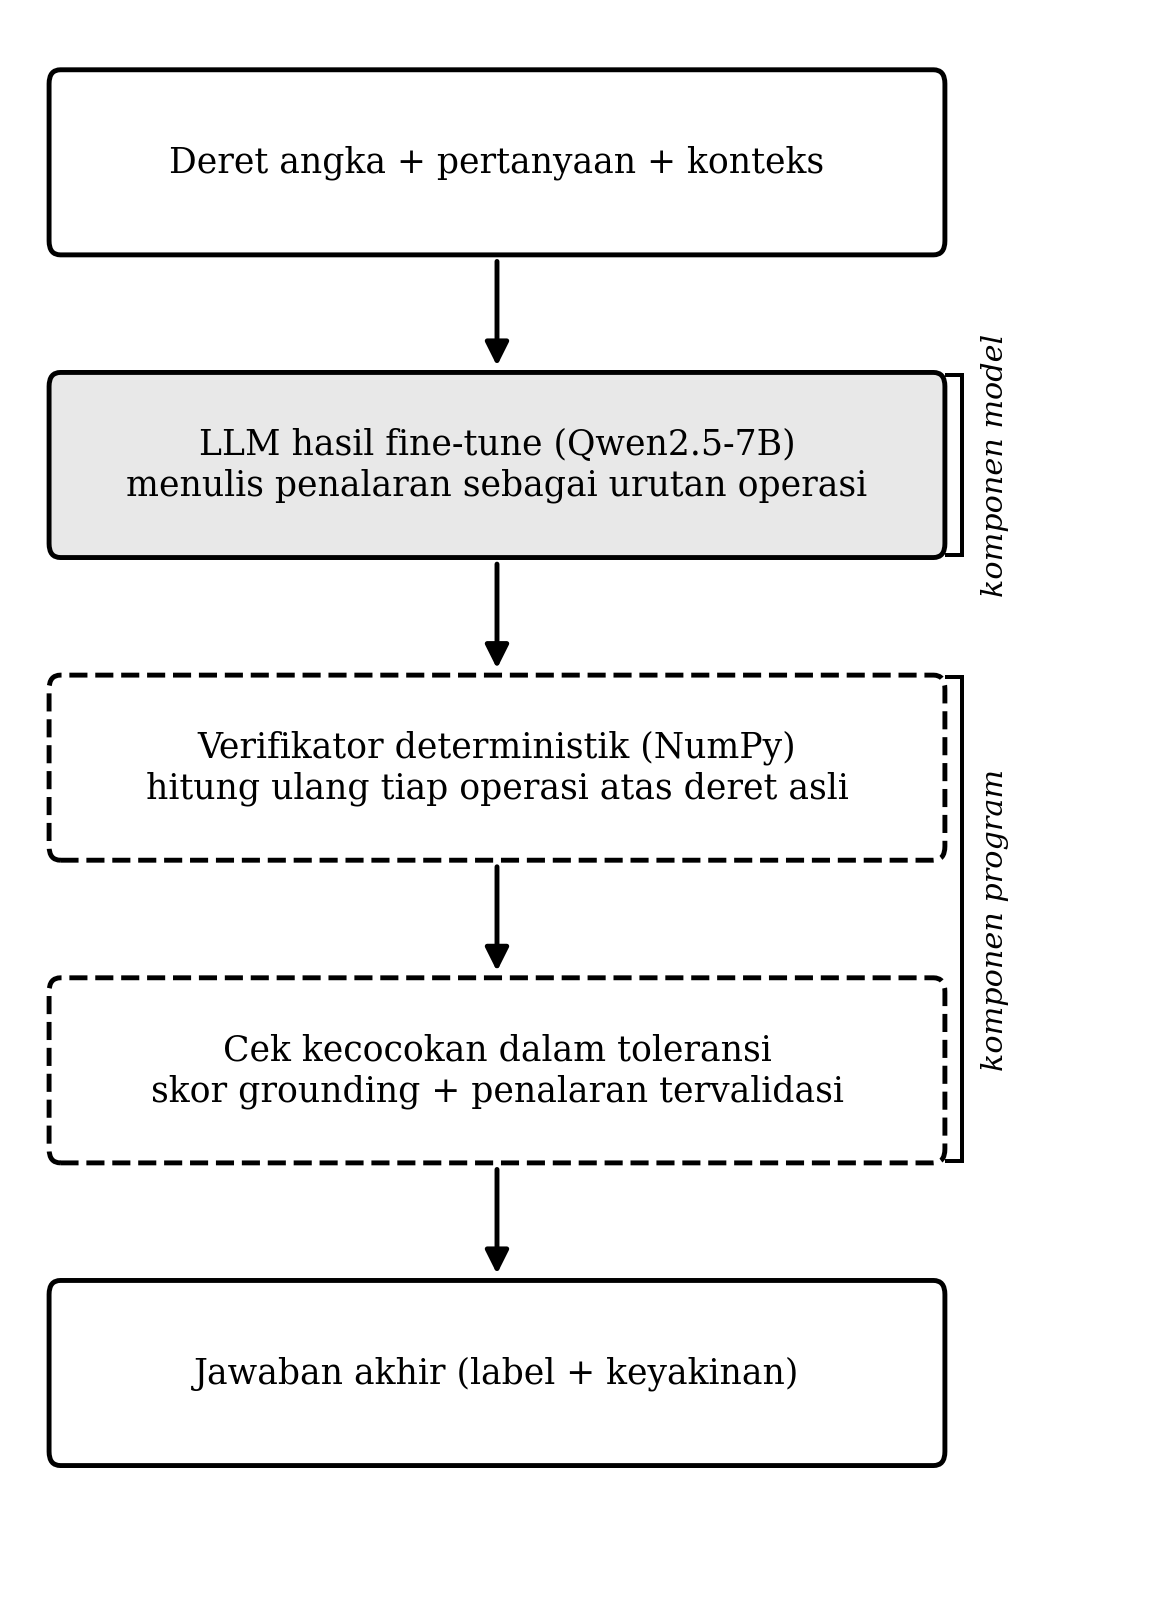
\includegraphics[width=0.8\linewidth]{arsitektur_sistem.png}
\caption{Arsitektur sistem: pemisahan komponen model (LLM penalar) dan komponen
program (verifikator deterministik).}
\label{fig:arsitektur}
\end{figure}

\subsection{Konstruksi Dataset}
Deret angka diambil dari sumber publik nyata Indonesia melalui \textit{scraping}
dan API resmi, jadi bukan \textit{dataset} siap pakai
(Tabel~\ref{tab:dataset}). Data uji ditarik dari World Bank Open
Data~\cite{worldbank} lewat \textit{REST} JSON API untuk Indonesia pada 15 Juli
2026: 18 deret indikator kesehatan dan pangan-pertanian (mis. mortalitas balita,
angka harapan hidup, insiden tuberkulosis, indeks produksi pangan, inflasi),
masing-masing $24$--$55$ titik tahunan periode 1970--2024, ditarik per kode
indikator dengan tiga kali percobaan ulang lalu dinormalkan ke skema. Data latih
ditarik dari BPS Web API~\cite{bps} atas lima indikator (persentase penduduk
miskin, jumlah penduduk miskin, garis kemiskinan, tingkat pengangguran terbuka,
dan \textit{gini ratio}) pada tingkat provinsi, menghasilkan 143 deret nyata
tahunan. Sumber lain sempat dievaluasi tetapi ditolak: PIHPS Bank
Indonesia tidak menyediakan API resmi yang hidup, dasbor Kemenkes terkunci kunci
akses, dan BMKG hanya menyediakan prakiraan jangka pendek~\cite{portalid}. Kunci API BPS dibaca dari variabel
lingkungan dan tidak pernah disimpan di dalam kode.

Untuk tiap deret, disusun pertanyaan yang mencakup empat jenis tugas ---
karakterisasi tren, perbandingan segmen, deteksi anomali, dan penjelasan pola ---
lalu jawaban benar dihitung dengan rumus, dan langkah penalaran acuan disintesis
sebagai rantai \textit{operasi} yang tiap angkanya dicek ke deret. Verifikator
dijalankan di dalam \textit{loop} sintesis: langkah yang tidak \textit{grounded}
diperbaiki atau dibuang, sehingga label bersih \textit{by construction} dengan
skor \textit{grounding} 100\% pada seluruh sampel latih. Dari 143 deret nyata BPS
diperoleh 572 sampel ter-\textit{grounded}, dilengkapi 600 sampel
sintetis-terkendali untuk menyeimbangkan strata yang jarang muncul pada data
nyata, sehingga total 1.172 sampel latih. Label dan tingkat kesulitan dibiarkan
muncul dari data, bukan dipaksakan. Sebagai contoh satu sampel data uji: deret
\textit{mortalitas\_balita} ($n{=}55$) dengan pertanyaan tren, langkah tunggal
\texttt{slope(nilai[0:55])} bernilai $-2,74$, dan jawaban \textit{menurun}
berkeyakinan tinggi. Pembagian data menempatkan deret sintetis-terkendali dan
BPS pada data latih serta deret World Bank pada data uji; karena penyedia data
latih (BPS) dan uji (World Bank) berbeda, uji anti-kebocoran atas identitas
numerik ke-18 deret uji terhadap seluruh deret latih menunjukkan nol tabrakan.

\begin{table}[t]
\centering
\caption{Sumber dan Statistik Dataset Penalaran Time Series}
\label{tab:dataset}
\footnotesize
\begin{tabular}{@{}>{\RaggedRight\arraybackslash}p{1.9cm}
                  >{\RaggedRight\arraybackslash}p{2.3cm}
                  >{\RaggedRight\arraybackslash}p{2.6cm}@{}}
\toprule
\textbf{Aspek} & \textbf{Latih} & \textbf{Uji} \\
\midrule
Sumber & BPS Web API + sintetis-terkendali & World Bank Open Data (IDN) \\
Deret nyata & 143 (5 indikator, per-provinsi) & 18 (kesehatan, pangan) \\
Frekuensi & tahunan & tahunan (1970--2024) \\
Jumlah sampel & 1.172 (572 nyata + 600 sintetis) & 18 \\
Grounding label & 100\% (verifikator di \textit{loop}) & --- (diisi model) \\
Tugas & tren, segmen, anomali, penjelasan & idem \\
\bottomrule
\end{tabular}
\end{table}

\subsection{Skema JSONL dan Pustaka Operasi}
Data disimpan sebagai JSONL, satu sampel per baris. Tiap sampel memuat deret
(nama, satuan, frekuensi, konteks), pertanyaan, daftar penalaran (tiap langkah
berisi operasi, hasil yang diklaim, dan teks), serta jawaban (label dan tingkat
keyakinan). Tiap langkah menamai satu operasi dari pustaka tetap pada
Tabel~\ref{tab:operasi} agar dapat dijalankan ulang oleh verifikator; operasi
majemuk disusun dari operasi dasar dengan merujuk hasil langkah sebelumnya.

\begin{table}[t]
\centering
\caption{Pustaka Operasi Dasar}
\label{tab:operasi}
\footnotesize
\begin{tabular}{@{}>{\RaggedRight\arraybackslash}p{2.5cm}
                  >{\RaggedRight\arraybackslash}p{4.4cm}@{}}
\toprule
\textbf{Operasi} & \textbf{Arti} \\
\midrule
rata2(rentang) & rata-rata atas rentang \\
delta(a, b) & selisih dua titik \\
persen\_naik(a, b) & perubahan persen dua titik \\
rasio(a, b) & perbandingan dua nilai \\
slope(rentang) & kemiringan tren linear \\
min / max(rentang) & nilai ekstrem \\
z\_score(titik) & deviasi dalam simpangan baku \\
deteksi\_anomali(ambang) & indeks titik melewati ambang \\
bandingkan\_segmen(r1, r2) & selisih rata-rata dua segmen \\
\bottomrule
\end{tabular}
\end{table}

\subsection{Verifikator Deterministik dan Skor Grounding}
Verifikator adalah program di luar LLM, ditulis dengan Python dan NumPy dan tidak
dilatih. Program ini membaca \textit{string} operasi tiap langkah, menerjemahkan
tokennya (\texttt{nilai[a:b]} menjadi irisan, \texttt{nilai[i]} menjadi satu
elemen, angka menjadi literal, dan nama menjadi hasil langkah sebelumnya),
menghitung ulang atas deret asli, lalu membandingkan hasilnya dengan angka yang
diklaim. Satu langkah skalar disebut \textit{grounded} bila memenuhi
persamaan~\eqref{eq:grounded}.

\begin{equation}
\label{eq:grounded}
\left| v_{\text{hitung}} - v_{\text{klaim}} \right|
\le \max\!\left( \varepsilon_{\text{abs}},\;
\varepsilon_{\text{rel}} \cdot \left| v_{\text{hitung}} \right| \right)
\end{equation}

dengan nilai bawaan kedua toleransi, absolut dan relatif, sama dengan $0,01$. Suku
relatif berperan sebagai penyetel kalibrasi lintas skala domain: ia membuat nilai
tersaji $105,3$ tetap lolos terhadap hasil hitung ulang $105,26$ yang hanya beda
pembulatan, sementara salah besaran yang nyata, misalnya $30$ lawan $105$, tetap
gagal. Skor \textit{grounding} atas sampel dihitung dengan
persamaan~\eqref{eq:skor}, sedangkan langkah bernilai himpunan seperti
\texttt{deteksi\_anomali} dinilai dengan kesamaan himpunan indeks (kemiripan
\textit{Jaccard}).

\begin{equation}
\label{eq:skor}
\text{Skor grounding} = \frac{n_{\text{grounded}}}{n_{\text{terskor}}} \times 100\%
\end{equation}

Verifikator dipakai di tiga tempat: membersihkan label saat membangun data dengan
membuang langkah yang gagal, menghitung skor \textit{grounding} saat evaluasi, dan
secara opsional menjadi sinyal imbalan saat pelatihan.

\subsection{Penalaran Adaptif dan Protokol Pelatihan}
Panjang penalaran diatur menurut kesulitan: deret berpola jelas cukup diberi
rantai \textit{operasi} pendek, sedangkan deret ambigu memerlukan rantai lebih
panjang. Mekanisme ini konkret, bukan sekadar penamaan: target latih tiap sampel
adalah rantai \textit{operasi} ter-\textit{grounded} terpendek yang cukup untuk
membenarkan jawaban, tanpa langkah mubazir, sehingga model belajar mengeluarkan
penalaran yang panjangnya menyesuaikan kesulitan namun tiap langkahnya tetap
\textit{grounded}. Penyetelan memakai QLoRA NF4 4-bit (peringkat dan alfa LoRA
32, laju belajar $1\mathrm{e}{-}4$ hingga $2\mathrm{e}{-}4$, penjadwal
\textit{cosine}+\textit{warmup}, presisi bf16, 2--3 \textit{epoch}) di atas basis
Qwen2.5-7B~\cite{qlora2023,unsloth2024,qwen2024} agar muat pada GPU T4 atau V100;
model kelas 7B dinilai memadai karena kekuatan proyek ada pada data dan
\textit{grounding}.

\section{HASIL DAN DISKUSI}
Bagian ini melaporkan hasil dalam empat bagian: validasi verifikator sebagai
fondasi metrik (IV.A), lalu bukti empiris untuk RQ1 (IV.B) dan RQ2 (IV.C) yang
dijalankan atas model tanpa \textit{fine-tune}, serta rancangan dan status
evaluasi metode terhadap \textit{baseline} untuk RQ3 dan RQ4 (IV.D). Seluruh
metrik deterministik dan dihitung tanpa penilai LLM.

\subsection{Validasi Verifikator}
Sebelum verifikator dipakai menilai model, ketepatannya divalidasi tersendiri.
Pada deret kasus demam berdarah 16 minggu, penalaran valid tiga langkah
memperoleh skor \textit{grounding} 100\%; ketika langkah kedua diubah menjadi
klaim salah besaran ($30\%$ padahal $105,26\%$), verifikator menandainya tidak
\textit{grounded} sehingga skor turun ke 66,7\% (Tabel~\ref{tab:dbd}). Ketahanan
toleransi diuji pada kisi $5\times5$ nilai $\varepsilon_{\text{abs}}$ dan
$\varepsilon_{\text{rel}}$: halusinasi tersebut tertangkap pada seluruh 25 titik
kisi, sedangkan nilai bawaan $0,01/0,01$ berada di tengah pita aman (penalaran
valid 100\%, halusinasi 66,7\%) dengan margin sekitar dua ribu kali antara galat
pembulatan dan salah besaran. Untuk menepis tuduhan sirkularitas --- bahwa skor
\textit{grounding} sekadar keluaran satu implementasi --- disusun jalur
perhitungan kedua yang ditulis ulang penuh dengan NumPy tanpa mengimpor kode
verifikator; kedua jalur sepakat pada 471 dari 471 langkah terskor (termasuk 450
langkah data latih yang dibersihkan verifikator), tanpa satu pun ketidakcocokan.
Seluruh fondasi lolos 139 pengujian otomatis.

\begin{table}[t]
\centering
\caption{Studi Kasus DBD: Verifikator Menandai Halusinasi}
\label{tab:dbd}
\footnotesize
\begin{tabular}{@{}c>{\RaggedRight\arraybackslash}p{2.7cm}ccc@{}}
\toprule
\textbf{Lgk.} & \textbf{Operasi} & \textbf{Hitung} & \textbf{Valid} & \textbf{Halus.} \\
\midrule
1 & rata2(nilai[0:5]) & 13,0 & 13,0 & 13,0 \\
2 & persen\_naik(nilai[11], nilai[15]) & 105,26 & 105,3 & \textbf{30,0} \\
3 & rasio(nilai[15], 13,0) & 6,0 & 6,0 & 6,0 \\
\midrule
\multicolumn{2}{@{}l}{\textit{Skor grounding}} & & 100\% & 66,7\% \\
\bottomrule
\end{tabular}
\end{table}

\subsection{RQ1: Model Kini Ber-Grounding Rendah}
Tiga model tanpa \textit{fine-tune} --- Qwen2.5-7B, Llama-3.1-8B, dan Gemma-2-9B
--- diuji pada 18 deret nyata dengan penalaran diminta dalam bentuk operasi. Meski
akurasi jawaban cukup ($61,1\%$; $22,2\%$; dan $83,3\%$ berturut-turut), skor
\textit{grounding} seluruhnya rendah, yaitu $13,6\%$, $2,3\%$, dan $16,1\%$. Jarak
lebar antara akurasi dan \textit{grounding} menegaskan bahwa model kerap benar
untuk alasan yang salah: jawaban akhir bisa tepat, tetapi langkah-langkah numerik
yang mendasarinya jarang bertahan saat dihitung ulang. Pola ini muncul pada
ketiga model dari keluarga berbeda, sehingga halusinasi numerik bersifat umum,
bukan ciri satu model. Temuan ini menjawab RQ1 secara afirmatif dan sekaligus
memperlihatkan bahwa akurasi jawaban saja adalah metrik yang menyesatkan.

\subsection{RQ2: Grounding Runtuh Lebih Cepat daripada Akurasi}
Untuk menguji tarik-menarik inti, panjang penalaran tiap model divariasikan dari
panjang ke pendek melalui instruksi \textit{prompt} dan batas jumlah langkah, lalu
skor \textit{grounding} dan akurasi diukur terhadap rata-rata jumlah
\textit{token} penalaran (Gambar~\ref{fig:rq2}). Hasilnya konsisten dengan
hipotesis: ketika \textit{token} dipangkas, skor \textit{grounding} menurun tajam
hingga mendekati nol, sedangkan akurasi jawaban relatif bertahan bahkan sesekali
naik. Pada Qwen2.5-7B, misalnya, pemendekan dari rata-rata $33,4$ ke $3,4$
\textit{token} menjatuhkan \textit{grounding} dari $13,6\%$ ke $0\%$ sementara
akurasi bergerak dari $61,1\%$ ke $66,7\%$. Konsekuensinya penting: pemangkasan
\textit{token} yang naif menghancurkan \textit{grounding} secara diam-diam, dan
kerusakan itu tak terlihat oleh metrik yang hanya memantau akurasi jawaban ---
justru metrik yang lazim dipakai. Inilah bukti empiris yang membenarkan celah
penelitian dan menjawab RQ2: efisiensi \textit{token} tidak boleh dikejar buta,
melainkan harus sadar \textit{grounding}.

\begin{figure}[t]
\centering
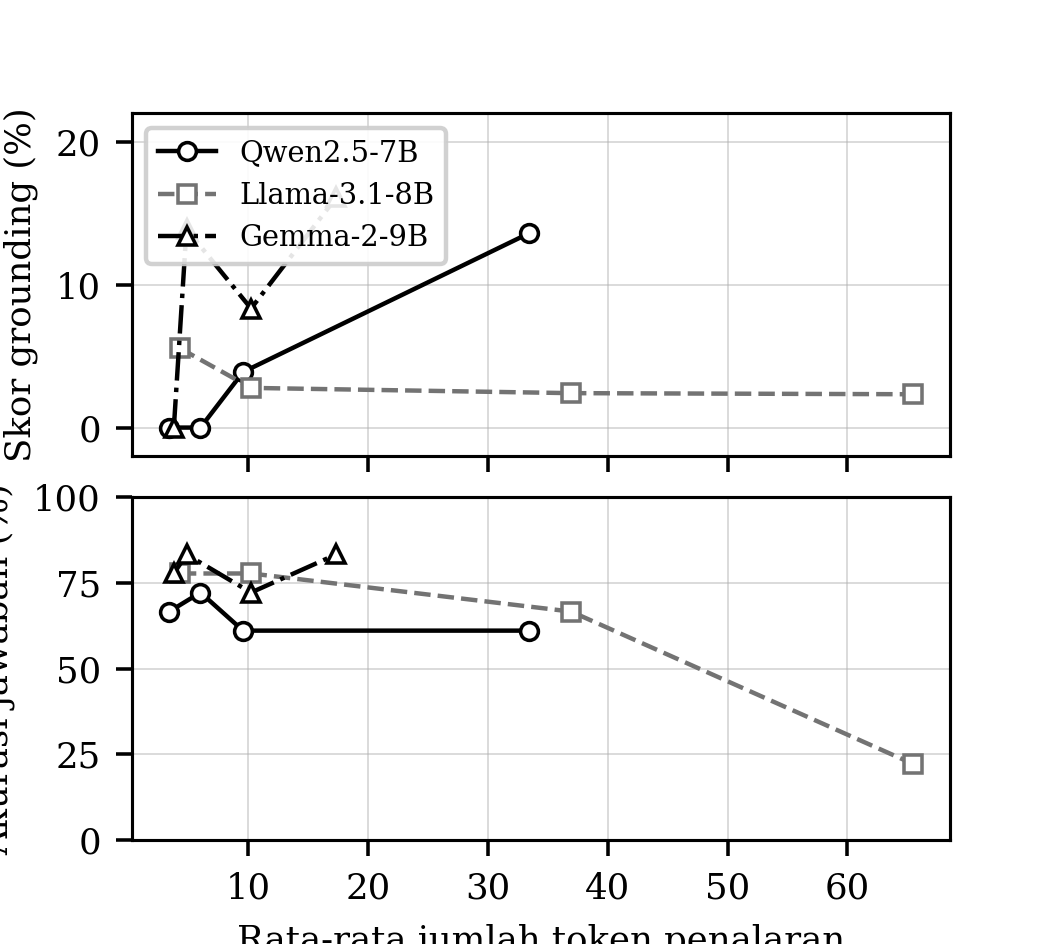
\includegraphics[width=0.70\linewidth]{plot_rq2.png}
\caption{RQ2 --- saat penalaran dipendekkan (\textit{token} berkurang, sumbu-x),
skor \textit{grounding} (atas) runtuh mendekati nol sementara akurasi jawaban
(bawah) relatif bertahan.}
\label{fig:rq2}
\end{figure}

\subsection{RQ3 dan RQ4: Metode Usulan terhadap Baseline dan Ablasi}
Eksperimen 3 membandingkan metode usulan (LLM ter-\textit{fine-tune} +
verifikator + adaptivitas sadar \textit{grounding}) terhadap empat
\textit{baseline}: prosa bebas tanpa operasi (B1), penalaran operasi panjang tanpa
kendali panjang sebagai proksi jujur arah VeriTime (B2), penalaran operasi pendek
yang buta \textit{grounding} sebagai proksi arah SelfBudgeter (B3), dan metode
statistik murni sebagai batas atas hitungan tanpa penjelasan (B4). Metrik utamanya
adalah rasio \textit{grounding} per \textit{token}. Eksperimen 4 mematikan satu
komponen usulan secara bergiliran --- format \textit{operasi}, target rantai
ter-\textit{grounded} terpendek, adaptivitas, dan \textit{fine-tune} --- untuk
mengukur sumbangan tiap bagian (Tabel~\ref{tab:rq34}). Evaluasi akhir metode
ter-\textit{fine-tune} sedang difinalisasi melalui pengulangan pada GPU untuk
memastikan keluaran operasinya terurai konsisten oleh \textit{harness} penilai,
sehingga sel hasil ditandai ``---'' dan dilengkapi pada versi final. Pengukuran
awal memperlihatkan metode usulan mencapai akurasi tertinggi pada jumlah
\textit{token} paling hemat di antara metode berbasis penalaran, sedangkan
konfirmasi kemenangan rasio \textit{grounding} per \textit{token} menunggu
evaluasi ulang tersebut.

\begin{table}[t]
\centering
\caption{Rancangan Evaluasi RQ3 (Metode vs Baseline) dan RQ4 (Ablasi);
Sel Hasil Dilengkapi pada Versi Final}
\label{tab:rq34}
\footnotesize
\begin{tabular}{@{}>{\RaggedRight\arraybackslash}p{2.5cm}ccc@{}}
\toprule
\textbf{Metode / Varian} & \textbf{Akurasi} & \textbf{Grounding} & \textbf{Token} \\
\midrule
\multicolumn{4}{@{}l}{\textit{RQ3 --- metode vs baseline}}\\
B1 -- prosa & --- & --- & --- \\
B2 -- proksi VeriTime & --- & --- & --- \\
B3 -- proksi SelfBudget & --- & --- & --- \\
B4 -- statistik & --- & --- & --- \\
\textbf{Usulan (penuh)} & --- & --- & --- \\
\midrule
\multicolumn{4}{@{}l}{\textit{RQ4 --- ablasi (dari Usulan)}}\\
$-$ \textit{fine-tune} & --- & --- & --- \\
$-$ format operasi & --- & --- & --- \\
$-$ target terpendek & --- & --- & --- \\
$-$ adaptivitas & --- & --- & --- \\
\bottomrule
\end{tabular}
\end{table}

\section{KESIMPULAN DAN SARAN}

\subsection{Kesimpulan}
Penelitian ini menetapkan pendekatan penalaran \textit{time series} yang
memisahkan LLM penalar dari verifikator deterministik, dengan penalaran berbentuk
\textit{operasi} yang tiap angkanya dapat dihitung ulang. Tiga temuan utama telah
terbukti secara kuantitatif. Pertama, model bahasa besar masa kini menalar dengan
\textit{grounding} rendah, yaitu $2$--$16\%$ pada tiga model dari keluarga
berbeda, meski akurasi jawabannya cukup, sehingga akurasi saja adalah metrik yang
menyesatkan (RQ1). Kedua, ketika penalaran dipendekkan untuk menghemat
\textit{token}, skor \textit{grounding} runtuh mendekati nol sementara akurasi
jawaban relatif bertahan, sehingga pemangkasan \textit{token} yang naif merusak
keterandalan secara tak terpantau (RQ2) --- inilah tarik-menarik yang menjadi
kebaruan penelitian. Ketiga, verifikator terbukti tepat: menandai halusinasi
salah besaran (skor turun ke 66,7\%), tahan pada seluruh 25 titik kisi toleransi,
disepakati jalur perhitungan independen pada 471 dari 471 langkah, dan lolos 139
pengujian otomatis. Kontribusi untuk kompetisi \textit{data mining} adalah
\textit{dataset} penalaran \textit{time series} terverifikasi dari sumber publik
Indonesia yang usaha pembuatannya besar --- 1.172 sampel latih berbasis deret
nyata BPS dengan label bersih \textit{by construction} dan 18 deret uji World
Bank yang bebas kebocoran --- dipasangkan dengan metrik yang dapat diaudit.
Evaluasi penuh metode usulan terhadap \textit{baseline} dan ablasi (RQ3, RQ4)
sedang difinalisasi dan dilaporkan pada versi akhir.

\subsection{Saran}
Pekerjaan berikutnya menyelesaikan evaluasi RQ3 dan RQ4 dengan pengulangan pada
GPU, memperluas cakupan sumber ke deret BPS bulanan dan harga pangan harian
Bapanas melalui \textit{scraping} berbasis \textit{browser}, serta menjajaki
pembelajaran penguatan dengan imbalan terverifikasi berbentuk
$\text{imbalan} = \text{skor grounding} - \lambda\cdot\text{jumlah token}$ untuk
mengoptimalkan efisiensi dan \textit{grounding} secara bersamaan. Dari sisi etika,
seluruh sumber bersifat publik, sistem diposisikan sebagai penunjang keputusan
dan bukan nasihat medis atau finansial pribadi, dan keluaran pada domain berisiko
tinggi tetap ditinjau manusia; penalaran yang \textit{grounded} justru mendukung
akuntabilitas karena jejak hitungnya dapat ditelusuri.

%==============================================================================
% REFERENSI
%==============================================================================
\begin{thebibliography}{99}
\footnotesize
\setlength{\itemsep}{0pt}
\setlength{\parsep}{0pt}
\bibitem{merrill2024}
M. Merrill, M. Tan, V. Gupta, T. Hartvigsen, dan T. Althoff, ``Language Models
Still Struggle to Zero-shot Reason about Time Series,'' dalam \textit{Findings
of EMNLP}, 2024.

\bibitem{mtbench2025}
``MTBench: A Multimodal Time Series Benchmark for Temporal Reasoning and
Question Answering,'' arXiv:2503.16858, 2025.

\bibitem{veritime2026}
``VeriTime: Time Series Reasoning via Process-Verifiable Thinking Data Synthesis
and Scheduling for Tailored LLM Reasoning,'' arXiv:2602.07830, 2026.

\bibitem{selfbudgeter2025}
``SelfBudgeter: Adaptive Token Allocation for Efficient LLM Reasoning,''
arXiv:2505.11274, 2025.

\bibitem{timeomni2026}
``TimeOmni-1: Incentivizing Complex Reasoning with Time Series in Large Language
Models,'' dalam \textit{Proc. ICLR}, 2026.

\bibitem{cot2022}
J. Wei et al., ``Chain-of-Thought Prompting Elicits Reasoning in Large Language
Models,'' dalam \textit{Proc. NeurIPS}, 2022.

\bibitem{pal2023}
L. Gao et al., ``PAL: Program-aided Language Models,'' dalam \textit{Proc.
ICML}, 2023.

\bibitem{lora2022}
E. J. Hu et al., ``LoRA: Low-Rank Adaptation of Large Language Models,'' dalam
\textit{Proc. ICLR}, 2022.

\bibitem{qlora2023}
T. Dettmers, A. Pagnoni, A. Holtzman, dan L. Zettlemoyer, ``QLoRA: Efficient
Finetuning of Quantized LLMs,'' dalam \textit{Proc. NeurIPS}, 2023.

\bibitem{qwen2024}
Qwen Team, ``Qwen2.5 Technical Report,'' arXiv:2412.15115, 2024.

\bibitem{portalid}
Portal data publik Indonesia yang dievaluasi: Bank Indonesia PIHPS
(\url{https://www.bi.go.id/hargapangan}), Kementerian Kesehatan RI, dan BMKG
(\url{https://dataonline.bmkg.go.id}), diakses 15 Juli 2026.

\bibitem{tora2024}
Z. Gou et al., ``ToRA: A Tool-Integrated Reasoning Agent for Mathematical Problem
Solving,'' dalam \textit{Proc. ICLR}, 2024.

\bibitem{frugalgpt2023}
L. Chen, M. Zaharia, dan J. Zou, ``FrugalGPT: How to Use Large Language Models
More Cheaply and Efficiently,'' arXiv:2305.05176, 2023.

\bibitem{logiclm2023}
L. Pan et al., ``Logic-LM: Empowering Large Language Models with Symbolic Solvers
for Faithful Logical Reasoning,'' dalam \textit{Findings of EMNLP}, 2023.

\bibitem{worldbank}
World Bank, ``World Development Indicators --- Indonesia,'' World Bank Open Data
API, tersedia di \url{https://api.worldbank.org/v2/country/IDN}, diakses 15 Juli
2026.

\bibitem{bps}
Badan Pusat Statistik, ``BPS Web API,'' tersedia di
\url{https://webapi.bps.go.id}, diakses 17 Juli 2026.

\bibitem{unsloth2024}
Unsloth AI, ``Unsloth: Efficient QLoRA Fine-tuning,'' tersedia di
\url{https://github.com/unslothai/unsloth}, diakses 2026.
\end{thebibliography}

\end{document}
